\documentclass[twoside]{book}

% Packages required by doxygen
\usepackage{fixltx2e}
\usepackage{calc}
\usepackage{doxygen}
\usepackage[export]{adjustbox} % also loads graphicx
\usepackage{graphicx}
\usepackage[utf8]{inputenc}
\usepackage{makeidx}
\usepackage{multicol}
\usepackage{multirow}
\PassOptionsToPackage{warn}{textcomp}
\usepackage{textcomp}
\usepackage[nointegrals]{wasysym}
\usepackage[table]{xcolor}

% Font selection
\usepackage[T1]{fontenc}
\usepackage[scaled=.90]{helvet}
\usepackage{courier}
\usepackage{amssymb}
\usepackage{sectsty}
\renewcommand{\familydefault}{\sfdefault}
\allsectionsfont{%
  \fontseries{bc}\selectfont%
  \color{darkgray}%
}
\renewcommand{\DoxyLabelFont}{%
  \fontseries{bc}\selectfont%
  \color{darkgray}%
}
\newcommand{\+}{\discretionary{\mbox{\scriptsize$\hookleftarrow$}}{}{}}

% Page & text layout
\usepackage{geometry}
\geometry{%
  a4paper,%
  top=2.5cm,%
  bottom=2.5cm,%
  left=2.5cm,%
  right=2.5cm%
}
\tolerance=750
\hfuzz=15pt
\hbadness=750
\setlength{\emergencystretch}{15pt}
\setlength{\parindent}{0cm}
\setlength{\parskip}{0.2cm}
\makeatletter
\renewcommand{\paragraph}{%
  \@startsection{paragraph}{4}{0ex}{-1.0ex}{1.0ex}{%
    \normalfont\normalsize\bfseries\SS@parafont%
  }%
}
\renewcommand{\subparagraph}{%
  \@startsection{subparagraph}{5}{0ex}{-1.0ex}{1.0ex}{%
    \normalfont\normalsize\bfseries\SS@subparafont%
  }%
}
\makeatother

% Headers & footers
\usepackage{fancyhdr}
\pagestyle{fancyplain}
\fancyhead[LE]{\fancyplain{}{\bfseries\thepage}}
\fancyhead[CE]{\fancyplain{}{}}
\fancyhead[RE]{\fancyplain{}{\bfseries\leftmark}}
\fancyhead[LO]{\fancyplain{}{\bfseries\rightmark}}
\fancyhead[CO]{\fancyplain{}{}}
\fancyhead[RO]{\fancyplain{}{\bfseries\thepage}}
\fancyfoot[LE]{\fancyplain{}{}}
\fancyfoot[CE]{\fancyplain{}{}}
\fancyfoot[RE]{\fancyplain{}{\bfseries\scriptsize Generated on Tue Nov 10 2015 10\+:32\+:52 for P\+C to Micro\+Master Application by Doxygen }}
\fancyfoot[LO]{\fancyplain{}{\bfseries\scriptsize Generated on Tue Nov 10 2015 10\+:32\+:52 for P\+C to Micro\+Master Application by Doxygen }}
\fancyfoot[CO]{\fancyplain{}{}}
\fancyfoot[RO]{\fancyplain{}{}}
\renewcommand{\footrulewidth}{0.4pt}
\renewcommand{\chaptermark}[1]{%
  \markboth{#1}{}%
}
\renewcommand{\sectionmark}[1]{%
  \markright{\thesection\ #1}%
}

% Indices & bibliography
\usepackage{natbib}
\usepackage[titles]{tocloft}
\setcounter{tocdepth}{3}
\setcounter{secnumdepth}{5}
\makeindex

% Hyperlinks (required, but should be loaded last)
\usepackage{ifpdf}
\ifpdf
  \usepackage[pdftex,pagebackref=true]{hyperref}
\else
  \usepackage[ps2pdf,pagebackref=true]{hyperref}
\fi
\hypersetup{%
  colorlinks=true,%
  linkcolor=blue,%
  citecolor=blue,%
  unicode%
}

% Custom commands
\newcommand{\clearemptydoublepage}{%
  \newpage{\pagestyle{empty}\cleardoublepage}%
}


%===== C O N T E N T S =====

\begin{document}

% Titlepage & ToC
\hypersetup{pageanchor=false,
             bookmarks=true,
             bookmarksnumbered=true,
             pdfencoding=unicode
            }
\pagenumbering{roman}
\begin{titlepage}
\vspace*{7cm}
\begin{center}%
{\Large P\+C to Micro\+Master Application \\[1ex]\large v1.\+04 }\\
\vspace*{1cm}
{\large Generated by Doxygen 1.8.10}\\
\vspace*{0.5cm}
{\small Tue Nov 10 2015 10:32:52}\\
\end{center}
\end{titlepage}
\clearemptydoublepage
\tableofcontents
\clearemptydoublepage
\pagenumbering{arabic}
\hypersetup{pageanchor=true}

%--- Begin generated contents ---
\chapter{Aquiring content of registers with the U\+S\+S-\/protocol}
\label{index}\hypertarget{index}{}u\+:\textbackslash{}6th\+\_\+semester

the main loop increases continuously a float value by 0.\+01 every 300 ms. then an array for the display is calculated in the display\+\_\+7\+\_\+segment() function. finally this array is being displayed in the I\+R\+Q routine, generated by a timer 0. 



 \begin{DoxyVersion}{Version}
1.\+3 
\end{DoxyVersion}
\begin{DoxyDate}{Date}
29.\+04.\+2015 
\end{DoxyDate}
\begin{DoxyAuthor}{Author}
pk 
\end{DoxyAuthor}

\chapter{This Page references to some documents about U\+S\+S protocol.}
\label{referenced_documents}
\hypertarget{referenced_documents}{}
\section{Links\+:}\label{referenced_documents_links_sec}
~\newline
 {\tt U\+S\+S2\+Lab\+V\+I\+E\+W.\+pdf} ~\newline
 {\tt Cykliczna i acykliczna komunikacja.\+pdf} ~\newline
 {\tt Doxygen tips} 
\chapter{File Index}
\section{File List}
Here is a list of all files with brief descriptions\+:\begin{DoxyCompactList}
\item\contentsline{section}{U\+:/\+I\+C\+T/7th\+\_\+semester/bpri2/code/my\+Ethernut/rs485/src/{\bf main.\+c} }{\pageref{main_8c}}{}
\item\contentsline{section}{U\+:/\+I\+C\+T/7th\+\_\+semester/bpri2/code/my\+Ethernut/rs485/src/{\bf my\+Memory.\+c} }{\pageref{my_memory_8c}}{}
\item\contentsline{section}{U\+:/\+I\+C\+T/7th\+\_\+semester/bpri2/code/my\+Ethernut/rs485/src/{\bf my\+Memory.\+h} }{\pageref{my_memory_8h}}{}
\item\contentsline{section}{U\+:/\+I\+C\+T/7th\+\_\+semester/bpri2/code/my\+Ethernut/rs485/src/{\bf my\+R\+T\+L.\+c} }{\pageref{my_r_t_l_8c}}{}
\item\contentsline{section}{U\+:/\+I\+C\+T/7th\+\_\+semester/bpri2/code/my\+Ethernut/rs485/src/{\bf my\+R\+T\+L.\+h} }{\pageref{my_r_t_l_8h}}{}
\item\contentsline{section}{U\+:/\+I\+C\+T/7th\+\_\+semester/bpri2/code/my\+Ethernut/rs485/src/{\bf my\+Trash.\+c} }{\pageref{my_trash_8c}}{}
\item\contentsline{section}{U\+:/\+I\+C\+T/7th\+\_\+semester/bpri2/code/my\+Ethernut/rs485/src/{\bf my\+Uart.\+c} }{\pageref{my_uart_8c}}{}
\item\contentsline{section}{U\+:/\+I\+C\+T/7th\+\_\+semester/bpri2/code/my\+Ethernut/rs485/src/{\bf my\+Uart.\+h} }{\pageref{my_uart_8h}}{}
\item\contentsline{section}{U\+:/\+I\+C\+T/7th\+\_\+semester/bpri2/code/my\+Ethernut/rs485/src/{\bf my\+Util.\+c} }{\pageref{my_util_8c}}{}
\item\contentsline{section}{U\+:/\+I\+C\+T/7th\+\_\+semester/bpri2/code/my\+Ethernut/rs485/src/{\bf my\+Util.\+h} }{\pageref{my_util_8h}}{}
\item\contentsline{section}{U\+:/\+I\+C\+T/7th\+\_\+semester/bpri2/code/my\+Ethernut/rs485/src/{\bf usscalc.\+c} }{\pageref{usscalc_8c}}{}
\item\contentsline{section}{U\+:/\+I\+C\+T/7th\+\_\+semester/bpri2/code/my\+Ethernut/rs485/src/{\bf usscalc.\+h} }{\pageref{usscalc_8h}}{}
\end{DoxyCompactList}

\chapter{File Documentation}
\hypertarget{main_8c}{}\doxysection{main.\+c File Reference}
\label{main_8c}\index{main.c@{main.c}}
{\ttfamily \#include $<$D\+A\+V\+E.\+h$>$}\newline
{\ttfamily \#include \char`\"{}Manager\+Task.\+h\char`\"{}}\newline
{\ttfamily \#include \char`\"{}Uart\+Task.\+h\char`\"{}}\newline
{\ttfamily \#include \char`\"{}Spi\+Task.\+h\char`\"{}}\newline
{\ttfamily \#include \char`\"{}Worker1\+Task.\+h\char`\"{}}\newline
{\ttfamily \#include \char`\"{}Worker2\+Task.\+h\char`\"{}}\newline
Include dependency graph for main.\+c\+:
\nopagebreak
\begin{figure}[H]
\begin{center}
\leavevmode
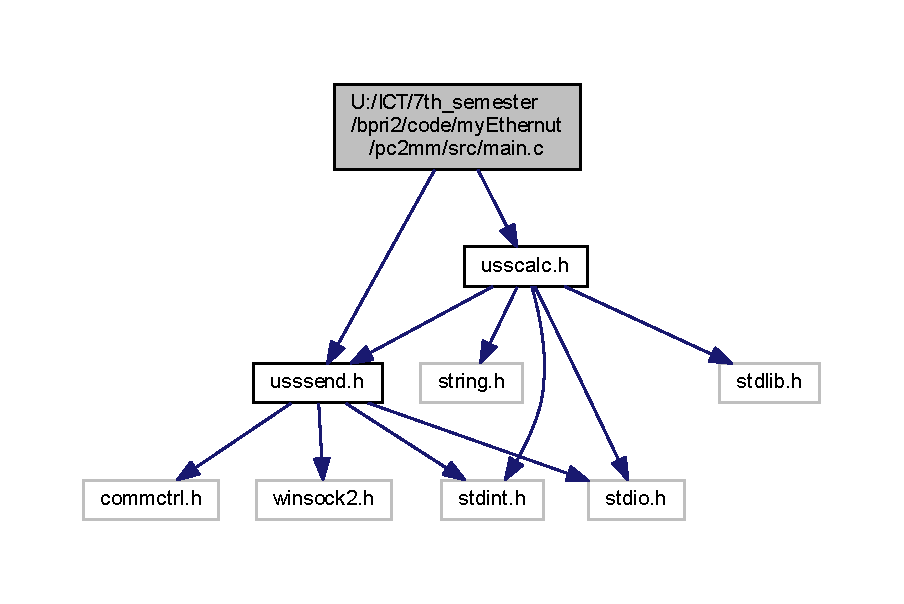
\includegraphics[width=350pt]{main_8c__incl}
\end{center}
\end{figure}
\doxysubsection*{Data Structures}
\begin{DoxyCompactItemize}
\item 
struct \mbox{\hyperlink{structparameter__struct}{parameter\+\_\+struct}}
\item 
struct \mbox{\hyperlink{struct_s_e_m_a_p_h_o_r_e___p_a_r_a_m_e_t_e_r_s}{S\+E\+M\+A\+P\+H\+O\+R\+E\+\_\+\+P\+A\+R\+A\+M\+E\+T\+E\+RS}}
\end{DoxyCompactItemize}
\doxysubsection*{Typedefs}
\begin{DoxyCompactItemize}
\item 
typedef struct \mbox{\hyperlink{structparameter__struct}{parameter\+\_\+struct}} \mbox{\hyperlink{main_8c_a4f866bc389d610b9af1569828c5cb796}{parameter\+\_\+struct\+\_\+t}}
\item 
typedef struct \mbox{\hyperlink{struct_s_e_m_a_p_h_o_r_e___p_a_r_a_m_e_t_e_r_s}{S\+E\+M\+A\+P\+H\+O\+R\+E\+\_\+\+P\+A\+R\+A\+M\+E\+T\+E\+RS}} \mbox{\hyperlink{main_8c_a8fa66a9bec224102af9be786a011d0ad}{x\+Semaphore\+Parameters\+\_\+t}}
\end{DoxyCompactItemize}
\doxysubsection*{Functions}
\begin{DoxyCompactItemize}
\item 
void \mbox{\hyperlink{main_8c_a0631242f9ef4df98c0aa08fc3477016b}{My\+L\+E\+Ds\+Toggling}} (uint8\+\_\+t tyle\+Razy)
\item 
void \mbox{\hyperlink{main_8c_a73549cfa09efe760d01971a22fd6b473}{My\+Error\+Handler}} (\mbox{\hyperlink{_generated_2_f_r_e_e_r_t_o_s_2task_8h_ae95f44d4cfeb4a599c6cc258d241cb6b}{Task\+Handle\+\_\+t}} x\+U\+A\+R\+T\+Handle)
\item 
void \mbox{\hyperlink{main_8c_a6a82a5f642a3795d49ee2a181494f472}{v\+Application\+Stack\+Overflow\+Hook}} (\mbox{\hyperlink{_model_2_a_p_p_s_2_f_r_e_e_r_t_o_s_2v4__1__2_2_templates_2_free_r_t_o_s_8h_af7cd8f53b62f0c497b442b504c30f2ec}{x\+Task\+Handle}} $\ast$px\+Task, signed char $\ast$pc\+Task\+Name)
\item 
void \mbox{\hyperlink{main_8c_a73f6aa45470ada02a5d6f3a522d8f13c}{v\+Application\+Malloc\+Failed\+Hook}} ()
\item 
void \mbox{\hyperlink{main_8c_afa643a0090e2cb938031a8ce2c46033c}{my\+Timer\+Callback}} (\mbox{\hyperlink{_model_2_a_p_p_s_2_f_r_e_e_r_t_o_s_2v4__1__2_2_templates_2_free_r_t_o_s_8h_a9fa57c444af781c3b6286f5cc9e4982d}{x\+Timer\+Handle}} px\+Timer)
\item 
int \mbox{\hyperlink{main_8c_a840291bc02cba5474a4cb46a9b9566fe}{main}} (void)
\end{DoxyCompactItemize}
\doxysubsection*{Variables}
\begin{DoxyCompactItemize}
\item 
\mbox{\hyperlink{_generated_2_f_r_e_e_r_t_o_s_2queue_8h_aaf19d499892a4ce1409326ece00f5264}{Queue\+Handle\+\_\+t}} \mbox{\hyperlink{main_8c_aa78b6121b7586233293fb6cba5e19206}{x\+Queue}} = N\+U\+LL
\item 
\mbox{\hyperlink{_model_2_a_p_p_s_2_f_r_e_e_r_t_o_s_2v4__1__2_2_templates_2_free_r_t_o_s_8h_a2b4ea2af4cc24db3cbd458722e96fa2f}{x\+Queue\+Handle}} \mbox{\hyperlink{main_8c_a1f474f190f107b23b637c1ec19339180}{Queue\+\_\+id}}
\item 
\mbox{\hyperlink{_model_2_a_p_p_s_2_f_r_e_e_r_t_o_s_2v4__1__2_2_templates_2_free_r_t_o_s_8h_a520d8cf032327581ece00e5bd8e03a75}{x\+Semaphore\+Handle}} \mbox{\hyperlink{main_8c_a518b536ed9bf3aae03f23de3ca80d69a}{notification\+\_\+semaphore}}
\item 
\mbox{\hyperlink{_model_2_a_p_p_s_2_f_r_e_e_r_t_o_s_2v4__1__2_2_templates_2_free_r_t_o_s_8h_a9fa57c444af781c3b6286f5cc9e4982d}{x\+Timer\+Handle}} \mbox{\hyperlink{main_8c_a02eac32cb5e7d9181d0197f353680c36}{Timer\+\_\+handle}}
\item 
\mbox{\hyperlink{_model_2_a_p_p_s_2_f_r_e_e_r_t_o_s_2v4__1__2_2_templates_2_free_r_t_o_s_8h_af7cd8f53b62f0c497b442b504c30f2ec}{x\+Task\+Handle}} \mbox{\hyperlink{main_8c_af9594ea483e4b18a36cc64c770a0b2a6}{U\+A\+R\+T\+Handle}} = N\+U\+LL
\item 
\mbox{\hyperlink{_model_2_a_p_p_s_2_f_r_e_e_r_t_o_s_2v4__1__2_2_templates_2_free_r_t_o_s_8h_af7cd8f53b62f0c497b442b504c30f2ec}{x\+Task\+Handle}} \mbox{\hyperlink{main_8c_aeb8570170354bebca19705854397cc75}{S\+P\+I\+Handle}} = N\+U\+LL
\item 
\mbox{\hyperlink{_model_2_a_p_p_s_2_f_r_e_e_r_t_o_s_2v4__1__2_2_templates_2_free_r_t_o_s_8h_af7cd8f53b62f0c497b442b504c30f2ec}{x\+Task\+Handle}} \mbox{\hyperlink{main_8c_a0322c8c10fc32d9da88dbb42525d11cd}{worker1\+\_\+id}}
\item 
\mbox{\hyperlink{_model_2_a_p_p_s_2_f_r_e_e_r_t_o_s_2v4__1__2_2_templates_2_free_r_t_o_s_8h_af7cd8f53b62f0c497b442b504c30f2ec}{x\+Task\+Handle}} \mbox{\hyperlink{main_8c_ae10999ad4b9b69ce410922e0a977066e}{worker2\+\_\+id}}
\end{DoxyCompactItemize}


\doxysubsection{Typedef Documentation}
\mbox{\Hypertarget{main_8c_a4f866bc389d610b9af1569828c5cb796}\label{main_8c_a4f866bc389d610b9af1569828c5cb796}} 
\index{main.c@{main.c}!parameter\_struct\_t@{parameter\_struct\_t}}
\index{parameter\_struct\_t@{parameter\_struct\_t}!main.c@{main.c}}
\doxysubsubsection{\texorpdfstring{parameter\_struct\_t}{parameter\_struct\_t}}
{\footnotesize\ttfamily typedef struct \mbox{\hyperlink{structparameter__struct}{parameter\+\_\+struct}} \mbox{\hyperlink{main_8c_a4f866bc389d610b9af1569828c5cb796}{parameter\+\_\+struct\+\_\+t}}}

\mbox{\Hypertarget{main_8c_a8fa66a9bec224102af9be786a011d0ad}\label{main_8c_a8fa66a9bec224102af9be786a011d0ad}} 
\index{main.c@{main.c}!xSemaphoreParameters\_t@{xSemaphoreParameters\_t}}
\index{xSemaphoreParameters\_t@{xSemaphoreParameters\_t}!main.c@{main.c}}
\doxysubsubsection{\texorpdfstring{xSemaphoreParameters\_t}{xSemaphoreParameters\_t}}
{\footnotesize\ttfamily typedef struct \mbox{\hyperlink{struct_s_e_m_a_p_h_o_r_e___p_a_r_a_m_e_t_e_r_s}{S\+E\+M\+A\+P\+H\+O\+R\+E\+\_\+\+P\+A\+R\+A\+M\+E\+T\+E\+RS}} \mbox{\hyperlink{main_8c_a8fa66a9bec224102af9be786a011d0ad}{x\+Semaphore\+Parameters\+\_\+t}}}



\doxysubsection{Function Documentation}
\mbox{\Hypertarget{main_8c_a840291bc02cba5474a4cb46a9b9566fe}\label{main_8c_a840291bc02cba5474a4cb46a9b9566fe}} 
\index{main.c@{main.c}!main@{main}}
\index{main@{main}!main.c@{main.c}}
\doxysubsubsection{\texorpdfstring{main()}{main()}}
{\footnotesize\ttfamily int main (\begin{DoxyParamCaption}\item[{void}]{ }\end{DoxyParamCaption})}



Definition at line 77 of file main.\+c.



References config\+M\+I\+N\+I\+M\+A\+L\+\_\+\+S\+T\+A\+C\+K\+\_\+\+S\+I\+ZE, D\+A\+V\+E\+\_\+\+Init(), D\+A\+V\+E\+\_\+\+S\+T\+A\+T\+U\+S\+\_\+\+S\+U\+C\+C\+E\+SS, Manager\+\_\+\+Task(), my\+Timer\+Callback(), pd\+T\+R\+UE, pv\+Port\+Malloc(), Queue\+\_\+id, Timer\+\_\+handle, tsk\+I\+D\+L\+E\+\_\+\+P\+R\+I\+O\+R\+I\+TY, v\+Task\+Start\+Scheduler(), worker1\+\_\+id, worker1\+\_\+task(), worker2\+\_\+id, worker2\+\_\+task(), X\+M\+C\+\_\+\+D\+E\+B\+UG, x\+Queue, x\+Timer\+Create(), and x\+Timer\+Start.

Here is the call graph for this function\+:
\nopagebreak
\begin{figure}[H]
\begin{center}
\leavevmode
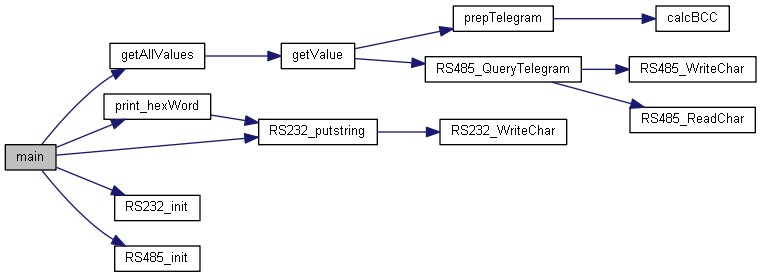
\includegraphics[width=350pt]{main_8c_a840291bc02cba5474a4cb46a9b9566fe_cgraph}
\end{center}
\end{figure}
\mbox{\Hypertarget{main_8c_a73549cfa09efe760d01971a22fd6b473}\label{main_8c_a73549cfa09efe760d01971a22fd6b473}} 
\index{main.c@{main.c}!MyErrorHandler@{MyErrorHandler}}
\index{MyErrorHandler@{MyErrorHandler}!main.c@{main.c}}
\doxysubsubsection{\texorpdfstring{MyErrorHandler()}{MyErrorHandler()}}
{\footnotesize\ttfamily void My\+Error\+Handler (\begin{DoxyParamCaption}\item[{\mbox{\hyperlink{_generated_2_f_r_e_e_r_t_o_s_2task_8h_ae95f44d4cfeb4a599c6cc258d241cb6b}{Task\+Handle\+\_\+t}}}]{x\+U\+A\+R\+T\+Handle }\end{DoxyParamCaption})}



Definition at line 42 of file main.\+c.



References My\+L\+E\+Ds\+Toggling(), pd\+M\+S\+\_\+\+T\+O\+\_\+\+T\+I\+C\+KS, v\+Task\+Delay(), and v\+Task\+Delete().

Here is the call graph for this function\+:
\nopagebreak
\begin{figure}[H]
\begin{center}
\leavevmode
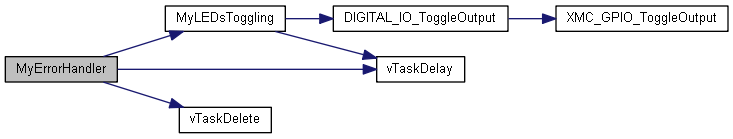
\includegraphics[width=350pt]{main_8c_a73549cfa09efe760d01971a22fd6b473_cgraph}
\end{center}
\end{figure}
\mbox{\Hypertarget{main_8c_a0631242f9ef4df98c0aa08fc3477016b}\label{main_8c_a0631242f9ef4df98c0aa08fc3477016b}} 
\index{main.c@{main.c}!MyLEDsToggling@{MyLEDsToggling}}
\index{MyLEDsToggling@{MyLEDsToggling}!main.c@{main.c}}
\doxysubsubsection{\texorpdfstring{MyLEDsToggling()}{MyLEDsToggling()}}
{\footnotesize\ttfamily void My\+L\+E\+Ds\+Toggling (\begin{DoxyParamCaption}\item[{uint8\+\_\+t}]{tyle\+Razy }\end{DoxyParamCaption})}



Definition at line 34 of file main.\+c.



References D\+I\+G\+I\+T\+A\+L\+\_\+\+I\+O\+\_\+\+Toggle\+Output(), L\+E\+D0, L\+E\+D1, and v\+Task\+Delay().



Referenced by My\+Error\+Handler(), v\+Application\+Malloc\+Failed\+Hook(), and v\+Application\+Stack\+Overflow\+Hook().

Here is the call graph for this function\+:
\nopagebreak
\begin{figure}[H]
\begin{center}
\leavevmode
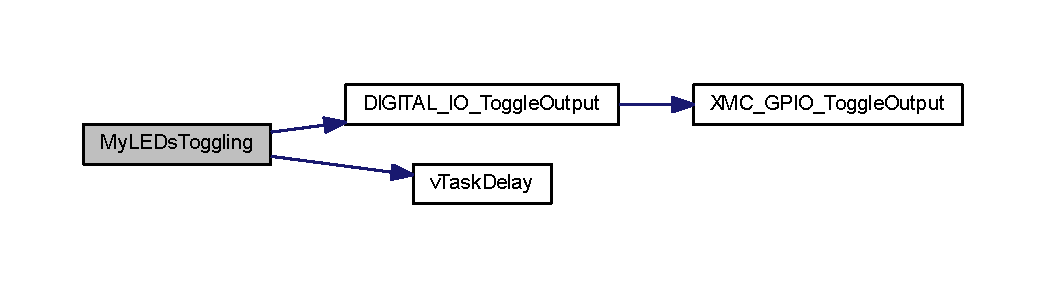
\includegraphics[width=350pt]{main_8c_a0631242f9ef4df98c0aa08fc3477016b_cgraph}
\end{center}
\end{figure}
\mbox{\Hypertarget{main_8c_afa643a0090e2cb938031a8ce2c46033c}\label{main_8c_afa643a0090e2cb938031a8ce2c46033c}} 
\index{main.c@{main.c}!myTimerCallback@{myTimerCallback}}
\index{myTimerCallback@{myTimerCallback}!main.c@{main.c}}
\doxysubsubsection{\texorpdfstring{myTimerCallback()}{myTimerCallback()}}
{\footnotesize\ttfamily void my\+Timer\+Callback (\begin{DoxyParamCaption}\item[{\mbox{\hyperlink{_model_2_a_p_p_s_2_f_r_e_e_r_t_o_s_2v4__1__2_2_templates_2_free_r_t_o_s_8h_a9fa57c444af781c3b6286f5cc9e4982d}{x\+Timer\+Handle}}}]{px\+Timer }\end{DoxyParamCaption})}



Definition at line 70 of file main.\+c.



References notification\+\_\+semaphore, and x\+Semaphore\+Give.



Referenced by main().

\mbox{\Hypertarget{main_8c_a73f6aa45470ada02a5d6f3a522d8f13c}\label{main_8c_a73f6aa45470ada02a5d6f3a522d8f13c}} 
\index{main.c@{main.c}!vApplicationMallocFailedHook@{vApplicationMallocFailedHook}}
\index{vApplicationMallocFailedHook@{vApplicationMallocFailedHook}!main.c@{main.c}}
\doxysubsubsection{\texorpdfstring{vApplicationMallocFailedHook()}{vApplicationMallocFailedHook()}}
{\footnotesize\ttfamily void v\+Application\+Malloc\+Failed\+Hook (\begin{DoxyParamCaption}{ }\end{DoxyParamCaption})}



Definition at line 63 of file main.\+c.



References My\+L\+E\+Ds\+Toggling(), pd\+M\+S\+\_\+\+T\+O\+\_\+\+T\+I\+C\+KS, and v\+Task\+Delay().



Referenced by pv\+Port\+Malloc().

Here is the call graph for this function\+:
\nopagebreak
\begin{figure}[H]
\begin{center}
\leavevmode
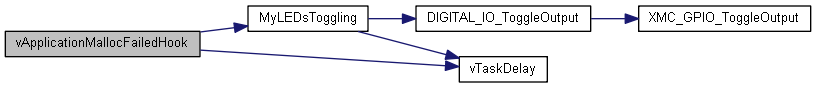
\includegraphics[width=350pt]{main_8c_a73f6aa45470ada02a5d6f3a522d8f13c_cgraph}
\end{center}
\end{figure}
\mbox{\Hypertarget{main_8c_a6a82a5f642a3795d49ee2a181494f472}\label{main_8c_a6a82a5f642a3795d49ee2a181494f472}} 
\index{main.c@{main.c}!vApplicationStackOverflowHook@{vApplicationStackOverflowHook}}
\index{vApplicationStackOverflowHook@{vApplicationStackOverflowHook}!main.c@{main.c}}
\doxysubsubsection{\texorpdfstring{vApplicationStackOverflowHook()}{vApplicationStackOverflowHook()}}
{\footnotesize\ttfamily void v\+Application\+Stack\+Overflow\+Hook (\begin{DoxyParamCaption}\item[{\mbox{\hyperlink{_model_2_a_p_p_s_2_f_r_e_e_r_t_o_s_2v4__1__2_2_templates_2_free_r_t_o_s_8h_af7cd8f53b62f0c497b442b504c30f2ec}{x\+Task\+Handle}} $\ast$}]{px\+Task,  }\item[{signed char $\ast$}]{pc\+Task\+Name }\end{DoxyParamCaption})}



Definition at line 53 of file main.\+c.



References My\+L\+E\+Ds\+Toggling(), pd\+M\+S\+\_\+\+T\+O\+\_\+\+T\+I\+C\+KS, and v\+Task\+Delay().

Here is the call graph for this function\+:
\nopagebreak
\begin{figure}[H]
\begin{center}
\leavevmode
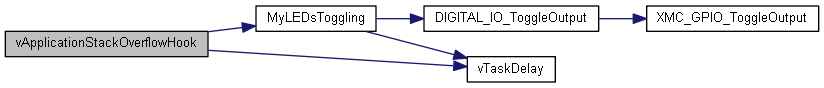
\includegraphics[width=350pt]{main_8c_a6a82a5f642a3795d49ee2a181494f472_cgraph}
\end{center}
\end{figure}


\doxysubsection{Variable Documentation}
\mbox{\Hypertarget{main_8c_a518b536ed9bf3aae03f23de3ca80d69a}\label{main_8c_a518b536ed9bf3aae03f23de3ca80d69a}} 
\index{main.c@{main.c}!notification\_semaphore@{notification\_semaphore}}
\index{notification\_semaphore@{notification\_semaphore}!main.c@{main.c}}
\doxysubsubsection{\texorpdfstring{notification\_semaphore}{notification\_semaphore}}
{\footnotesize\ttfamily \mbox{\hyperlink{_model_2_a_p_p_s_2_f_r_e_e_r_t_o_s_2v4__1__2_2_templates_2_free_r_t_o_s_8h_a520d8cf032327581ece00e5bd8e03a75}{x\+Semaphore\+Handle}} notification\+\_\+semaphore}



Definition at line 15 of file main.\+c.



Referenced by Manager\+\_\+\+Task(), and my\+Timer\+Callback().

\mbox{\Hypertarget{main_8c_a1f474f190f107b23b637c1ec19339180}\label{main_8c_a1f474f190f107b23b637c1ec19339180}} 
\index{main.c@{main.c}!Queue\_id@{Queue\_id}}
\index{Queue\_id@{Queue\_id}!main.c@{main.c}}
\doxysubsubsection{\texorpdfstring{Queue\_id}{Queue\_id}}
{\footnotesize\ttfamily \mbox{\hyperlink{_model_2_a_p_p_s_2_f_r_e_e_r_t_o_s_2v4__1__2_2_templates_2_free_r_t_o_s_8h_a2b4ea2af4cc24db3cbd458722e96fa2f}{x\+Queue\+Handle}} Queue\+\_\+id}



Definition at line 14 of file main.\+c.



Referenced by main(), Manager\+\_\+\+Task(), worker1\+\_\+task(), and worker2\+\_\+task().

\mbox{\Hypertarget{main_8c_aeb8570170354bebca19705854397cc75}\label{main_8c_aeb8570170354bebca19705854397cc75}} 
\index{main.c@{main.c}!SPIHandle@{SPIHandle}}
\index{SPIHandle@{SPIHandle}!main.c@{main.c}}
\doxysubsubsection{\texorpdfstring{SPIHandle}{SPIHandle}}
{\footnotesize\ttfamily \mbox{\hyperlink{_model_2_a_p_p_s_2_f_r_e_e_r_t_o_s_2v4__1__2_2_templates_2_free_r_t_o_s_8h_af7cd8f53b62f0c497b442b504c30f2ec}{x\+Task\+Handle}} S\+P\+I\+Handle = N\+U\+LL}



Definition at line 18 of file main.\+c.

\mbox{\Hypertarget{main_8c_a02eac32cb5e7d9181d0197f353680c36}\label{main_8c_a02eac32cb5e7d9181d0197f353680c36}} 
\index{main.c@{main.c}!Timer\_handle@{Timer\_handle}}
\index{Timer\_handle@{Timer\_handle}!main.c@{main.c}}
\doxysubsubsection{\texorpdfstring{Timer\_handle}{Timer\_handle}}
{\footnotesize\ttfamily \mbox{\hyperlink{_model_2_a_p_p_s_2_f_r_e_e_r_t_o_s_2v4__1__2_2_templates_2_free_r_t_o_s_8h_a9fa57c444af781c3b6286f5cc9e4982d}{x\+Timer\+Handle}} Timer\+\_\+handle}



Definition at line 16 of file main.\+c.



Referenced by main().

\mbox{\Hypertarget{main_8c_af9594ea483e4b18a36cc64c770a0b2a6}\label{main_8c_af9594ea483e4b18a36cc64c770a0b2a6}} 
\index{main.c@{main.c}!UARTHandle@{UARTHandle}}
\index{UARTHandle@{UARTHandle}!main.c@{main.c}}
\doxysubsubsection{\texorpdfstring{UARTHandle}{UARTHandle}}
{\footnotesize\ttfamily \mbox{\hyperlink{_model_2_a_p_p_s_2_f_r_e_e_r_t_o_s_2v4__1__2_2_templates_2_free_r_t_o_s_8h_af7cd8f53b62f0c497b442b504c30f2ec}{x\+Task\+Handle}} U\+A\+R\+T\+Handle = N\+U\+LL}



Definition at line 17 of file main.\+c.

\mbox{\Hypertarget{main_8c_a0322c8c10fc32d9da88dbb42525d11cd}\label{main_8c_a0322c8c10fc32d9da88dbb42525d11cd}} 
\index{main.c@{main.c}!worker1\_id@{worker1\_id}}
\index{worker1\_id@{worker1\_id}!main.c@{main.c}}
\doxysubsubsection{\texorpdfstring{worker1\_id}{worker1\_id}}
{\footnotesize\ttfamily \mbox{\hyperlink{_model_2_a_p_p_s_2_f_r_e_e_r_t_o_s_2v4__1__2_2_templates_2_free_r_t_o_s_8h_af7cd8f53b62f0c497b442b504c30f2ec}{x\+Task\+Handle}} worker1\+\_\+id}



Definition at line 19 of file main.\+c.



Referenced by main(), Manager\+\_\+\+Task(), and worker1\+\_\+task().

\mbox{\Hypertarget{main_8c_ae10999ad4b9b69ce410922e0a977066e}\label{main_8c_ae10999ad4b9b69ce410922e0a977066e}} 
\index{main.c@{main.c}!worker2\_id@{worker2\_id}}
\index{worker2\_id@{worker2\_id}!main.c@{main.c}}
\doxysubsubsection{\texorpdfstring{worker2\_id}{worker2\_id}}
{\footnotesize\ttfamily \mbox{\hyperlink{_model_2_a_p_p_s_2_f_r_e_e_r_t_o_s_2v4__1__2_2_templates_2_free_r_t_o_s_8h_af7cd8f53b62f0c497b442b504c30f2ec}{x\+Task\+Handle}} worker2\+\_\+id}



Definition at line 20 of file main.\+c.



Referenced by main(), Manager\+\_\+\+Task(), and worker2\+\_\+task().

\mbox{\Hypertarget{main_8c_aa78b6121b7586233293fb6cba5e19206}\label{main_8c_aa78b6121b7586233293fb6cba5e19206}} 
\index{main.c@{main.c}!xQueue@{xQueue}}
\index{xQueue@{xQueue}!main.c@{main.c}}
\doxysubsubsection{\texorpdfstring{xQueue}{xQueue}}
{\footnotesize\ttfamily \mbox{\hyperlink{_generated_2_f_r_e_e_r_t_o_s_2queue_8h_aaf19d499892a4ce1409326ece00f5264}{Queue\+Handle\+\_\+t}} x\+Queue = N\+U\+LL}



Definition at line 13 of file main.\+c.



Referenced by main(), pc\+Queue\+Get\+Name(), S\+P\+I\+\_\+\+Slave\+\_\+\+Task(), U\+A\+R\+T\+\_\+\+Task(), uc\+Queue\+Get\+Queue\+Type(), ux\+Queue\+Get\+Queue\+Number(), ux\+Queue\+Messages\+Waiting(), ux\+Queue\+Messages\+Waiting\+From\+I\+S\+R(), ux\+Queue\+Spaces\+Available(), v\+Queue\+Add\+To\+Registry(), v\+Queue\+Delete(), v\+Queue\+Set\+Queue\+Number(), v\+Queue\+Unregister\+Queue(), v\+Queue\+Wait\+For\+Message\+Restricted(), x\+Queue\+Generic\+Reset(), x\+Queue\+Generic\+Send(), x\+Queue\+Generic\+Send\+From\+I\+S\+R(), x\+Queue\+Give\+From\+I\+S\+R(), x\+Queue\+Is\+Queue\+Empty\+From\+I\+S\+R(), x\+Queue\+Is\+Queue\+Full\+From\+I\+S\+R(), x\+Queue\+Peek(), x\+Queue\+Peek\+From\+I\+S\+R(), x\+Queue\+Receive(), x\+Queue\+Receive\+From\+I\+S\+R(), and x\+Queue\+Semaphore\+Take().


\hypertarget{smietnik_8c}{}\section{U\+:/\+I\+C\+T/7th\+\_\+semester/bpri2/code/my\+Ethernut/pc2mm/src/smietnik.c File Reference}
\label{smietnik_8c}\index{U\+:/\+I\+C\+T/7th\+\_\+semester/bpri2/code/my\+Ethernut/pc2mm/src/smietnik.\+c@{U\+:/\+I\+C\+T/7th\+\_\+semester/bpri2/code/my\+Ethernut/pc2mm/src/smietnik.\+c}}

\section{U\+:/\+I\+C\+T/7th\+\_\+semester/bpri2/code/my\+Ethernut/rs485/src/usscalc.c File Reference}
\label{usscalc_8c}\index{U\+:/\+I\+C\+T/7th\+\_\+semester/bpri2/code/my\+Ethernut/rs485/src/usscalc.\+c@{U\+:/\+I\+C\+T/7th\+\_\+semester/bpri2/code/my\+Ethernut/rs485/src/usscalc.\+c}}
{\ttfamily \#include \char`\"{}usscalc.\+h\char`\"{}}\\*
Include dependency graph for usscalc.\+c\+:\nopagebreak
\begin{figure}[H]
\begin{center}
\leavevmode
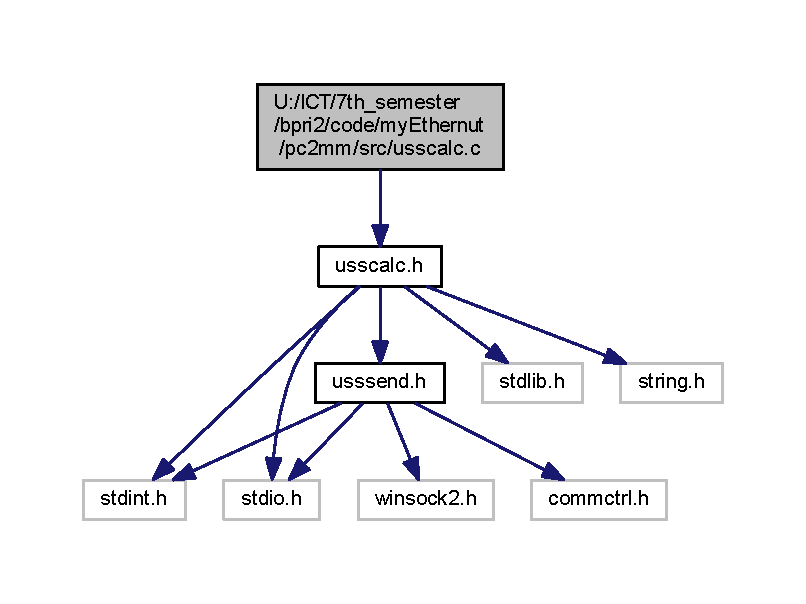
\includegraphics[width=162pt]{usscalc_8c__incl}
\end{center}
\end{figure}
\subsection*{Macros}
\begin{DoxyCompactItemize}
\item 
\#define {\bf ppo}~1
\item 
\#define {\bf mirror}~0
\item 
\#define {\bf pkw}~0
\item 
\#define {\bf A\+K}~0x00
\item 
\#define {\bf S\+P}~0
\item 
\#define {\bf P\+N\+U}~0x12bc
\item 
\#define {\bf P\+N\+Uex}~0x00
\item 
\#define {\bf I\+D\+X}~0x00
\end{DoxyCompactItemize}
\subsection*{Functions}
\begin{DoxyCompactItemize}
\item 
uint8\+\_\+t {\bf calc\+B\+C\+C} ()
\item 
void {\bf prep\+Telegram} (uint16\+\_\+t my\+Param)
\item 
uint16\+\_\+t {\bf get\+Value} (uint16\+\_\+t my\+Param)
\item 
void {\bf get\+All\+Values} (uint16\+\_\+t $\ast$mm\+Parameters\+Arr, uint8\+\_\+t length)
\end{DoxyCompactItemize}


\subsection{Macro Definition Documentation}
\index{usscalc.\+c@{usscalc.\+c}!A\+K@{A\+K}}
\index{A\+K@{A\+K}!usscalc.\+c@{usscalc.\+c}}
\subsubsection[{A\+K}]{\setlength{\rightskip}{0pt plus 5cm}\#define A\+K~0x00}\label{usscalc_8c_ac3a341ede33bbed651abe7f847361a6e}


Definition at line 29 of file usscalc.\+c.



Referenced by prep\+Telegram().

\index{usscalc.\+c@{usscalc.\+c}!I\+D\+X@{I\+D\+X}}
\index{I\+D\+X@{I\+D\+X}!usscalc.\+c@{usscalc.\+c}}
\subsubsection[{I\+D\+X}]{\setlength{\rightskip}{0pt plus 5cm}\#define I\+D\+X~0x00}\label{usscalc_8c_a223697fc2f8a4423171d86ced5c8872b}


Definition at line 41 of file usscalc.\+c.



Referenced by prep\+Telegram().

\index{usscalc.\+c@{usscalc.\+c}!mirror@{mirror}}
\index{mirror@{mirror}!usscalc.\+c@{usscalc.\+c}}
\subsubsection[{mirror}]{\setlength{\rightskip}{0pt plus 5cm}\#define mirror~0}\label{usscalc_8c_ab75be13d6d9ba70e2a9591121b408184}


Definition at line 20 of file usscalc.\+c.



Referenced by prep\+Telegram().

\index{usscalc.\+c@{usscalc.\+c}!pkw@{pkw}}
\index{pkw@{pkw}!usscalc.\+c@{usscalc.\+c}}
\subsubsection[{pkw}]{\setlength{\rightskip}{0pt plus 5cm}\#define pkw~0}\label{usscalc_8c_a0b9a09dbc3e3871baf2f518b82686dcb}


Definition at line 22 of file usscalc.\+c.

\index{usscalc.\+c@{usscalc.\+c}!P\+N\+U@{P\+N\+U}}
\index{P\+N\+U@{P\+N\+U}!usscalc.\+c@{usscalc.\+c}}
\subsubsection[{P\+N\+U}]{\setlength{\rightskip}{0pt plus 5cm}\#define P\+N\+U~0x12bc}\label{usscalc_8c_ab765f8aafdcbbd05cfcd27e208eb55b2}


Definition at line 35 of file usscalc.\+c.

\index{usscalc.\+c@{usscalc.\+c}!P\+N\+Uex@{P\+N\+Uex}}
\index{P\+N\+Uex@{P\+N\+Uex}!usscalc.\+c@{usscalc.\+c}}
\subsubsection[{P\+N\+Uex}]{\setlength{\rightskip}{0pt plus 5cm}\#define P\+N\+Uex~0x00}\label{usscalc_8c_a544eab7def9683a65c07c12fb091acc7}


Definition at line 38 of file usscalc.\+c.

\index{usscalc.\+c@{usscalc.\+c}!ppo@{ppo}}
\index{ppo@{ppo}!usscalc.\+c@{usscalc.\+c}}
\subsubsection[{ppo}]{\setlength{\rightskip}{0pt plus 5cm}\#define ppo~1}\label{usscalc_8c_a8ef3f4ce9afc84a8f4b4c62237ad2dcb}


Definition at line 18 of file usscalc.\+c.

\index{usscalc.\+c@{usscalc.\+c}!S\+P@{S\+P}}
\index{S\+P@{S\+P}!usscalc.\+c@{usscalc.\+c}}
\subsubsection[{S\+P}]{\setlength{\rightskip}{0pt plus 5cm}\#define S\+P~0}\label{usscalc_8c_aecd69d9a67487cc45c38eb184c50538a}


Definition at line 32 of file usscalc.\+c.



Referenced by prep\+Telegram().



\subsection{Function Documentation}
\index{usscalc.\+c@{usscalc.\+c}!calc\+B\+C\+C@{calc\+B\+C\+C}}
\index{calc\+B\+C\+C@{calc\+B\+C\+C}!usscalc.\+c@{usscalc.\+c}}
\subsubsection[{calc\+B\+C\+C()}]{\setlength{\rightskip}{0pt plus 5cm}uint8\+\_\+t calc\+B\+C\+C (
\begin{DoxyParamCaption}
{}
\end{DoxyParamCaption}
)}\label{usscalc_8c_a3758bfbaa4494e65cabf188a026502de}


Definition at line 43 of file usscalc.\+c.



References my\+Telegram.



Referenced by prep\+Telegram().

\index{usscalc.\+c@{usscalc.\+c}!get\+All\+Values@{get\+All\+Values}}
\index{get\+All\+Values@{get\+All\+Values}!usscalc.\+c@{usscalc.\+c}}
\subsubsection[{get\+All\+Values(uint16\+\_\+t $\ast$mm\+Parameters\+Arr, uint8\+\_\+t length)}]{\setlength{\rightskip}{0pt plus 5cm}void get\+All\+Values (
\begin{DoxyParamCaption}
\item[{uint16\+\_\+t $\ast$}]{mm\+Parameters\+Arr, }
\item[{uint8\+\_\+t}]{length}
\end{DoxyParamCaption}
)}\label{usscalc_8c_a0e6157d1764f0cd0bfd6895d2888d0f1}


Definition at line 106 of file usscalc.\+c.



References get\+Value().



Referenced by main().



Here is the call graph for this function\+:\nopagebreak
\begin{figure}[H]
\begin{center}
\leavevmode
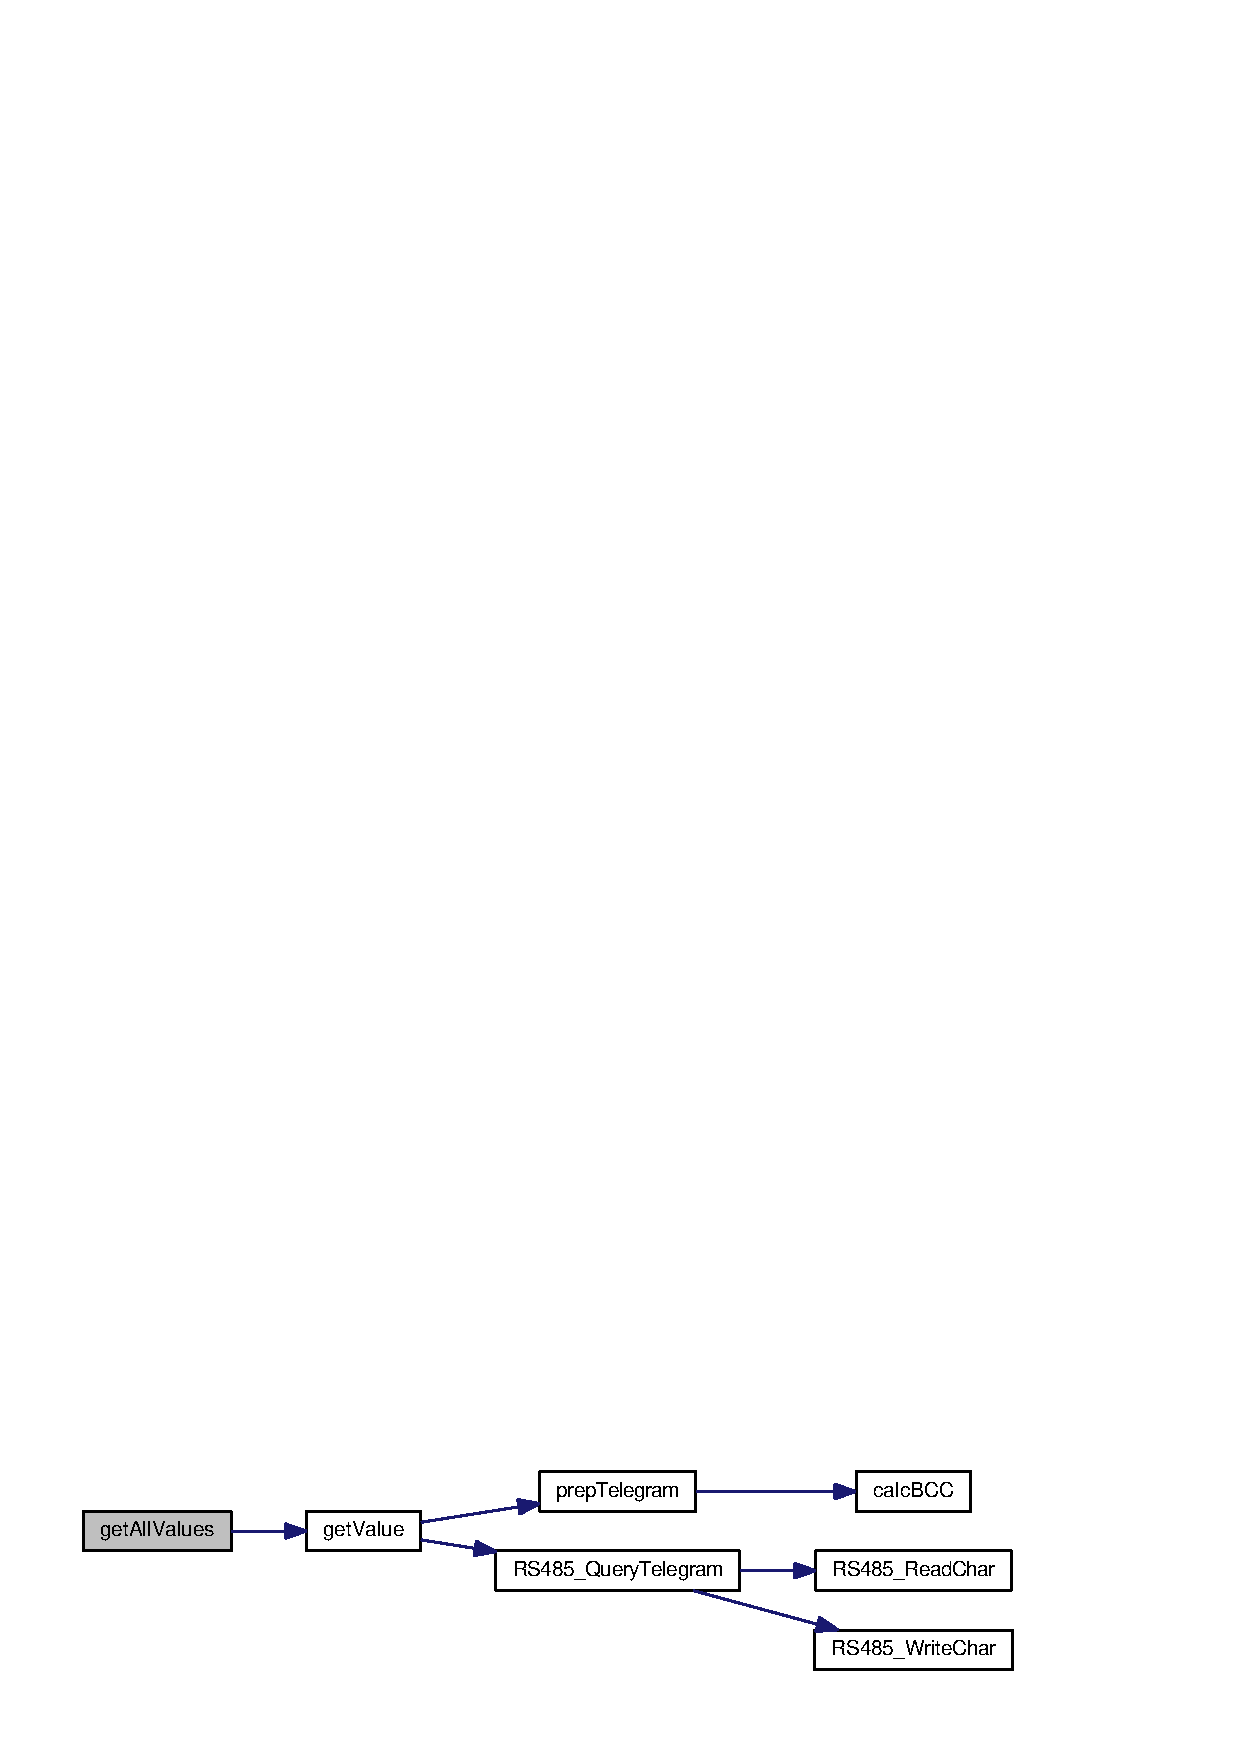
\includegraphics[width=350pt]{usscalc_8c_a0e6157d1764f0cd0bfd6895d2888d0f1_cgraph}
\end{center}
\end{figure}


\index{usscalc.\+c@{usscalc.\+c}!get\+Value@{get\+Value}}
\index{get\+Value@{get\+Value}!usscalc.\+c@{usscalc.\+c}}
\subsubsection[{get\+Value(uint16\+\_\+t my\+Param)}]{\setlength{\rightskip}{0pt plus 5cm}uint16\+\_\+t get\+Value (
\begin{DoxyParamCaption}
\item[{uint16\+\_\+t}]{my\+Param}
\end{DoxyParamCaption}
)}\label{usscalc_8c_a0d092db893cddedce1266d2971f2cd7f}


Definition at line 100 of file usscalc.\+c.



References my\+Telegram, prep\+Telegram(), and R\+S485\+\_\+\+Query\+Telegram().



Referenced by get\+All\+Values().



Here is the call graph for this function\+:\nopagebreak
\begin{figure}[H]
\begin{center}
\leavevmode
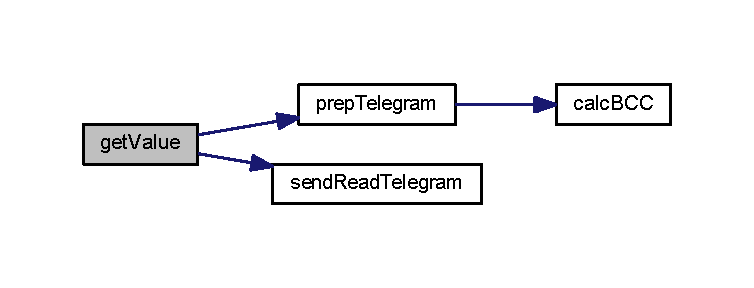
\includegraphics[width=350pt]{usscalc_8c_a0d092db893cddedce1266d2971f2cd7f_cgraph}
\end{center}
\end{figure}


\index{usscalc.\+c@{usscalc.\+c}!prep\+Telegram@{prep\+Telegram}}
\index{prep\+Telegram@{prep\+Telegram}!usscalc.\+c@{usscalc.\+c}}
\subsubsection[{prep\+Telegram(uint16\+\_\+t my\+Param)}]{\setlength{\rightskip}{0pt plus 5cm}void prep\+Telegram (
\begin{DoxyParamCaption}
\item[{uint16\+\_\+t}]{my\+Param}
\end{DoxyParamCaption}
)}\label{usscalc_8c_ac734b72553a80042ac173bfebf6b5185}


Definition at line 55 of file usscalc.\+c.



References A\+K, calc\+B\+C\+C(), I\+D\+X, mirror, my\+Telegram, and S\+P.



Referenced by get\+Value().



Here is the call graph for this function\+:\nopagebreak
\begin{figure}[H]
\begin{center}
\leavevmode
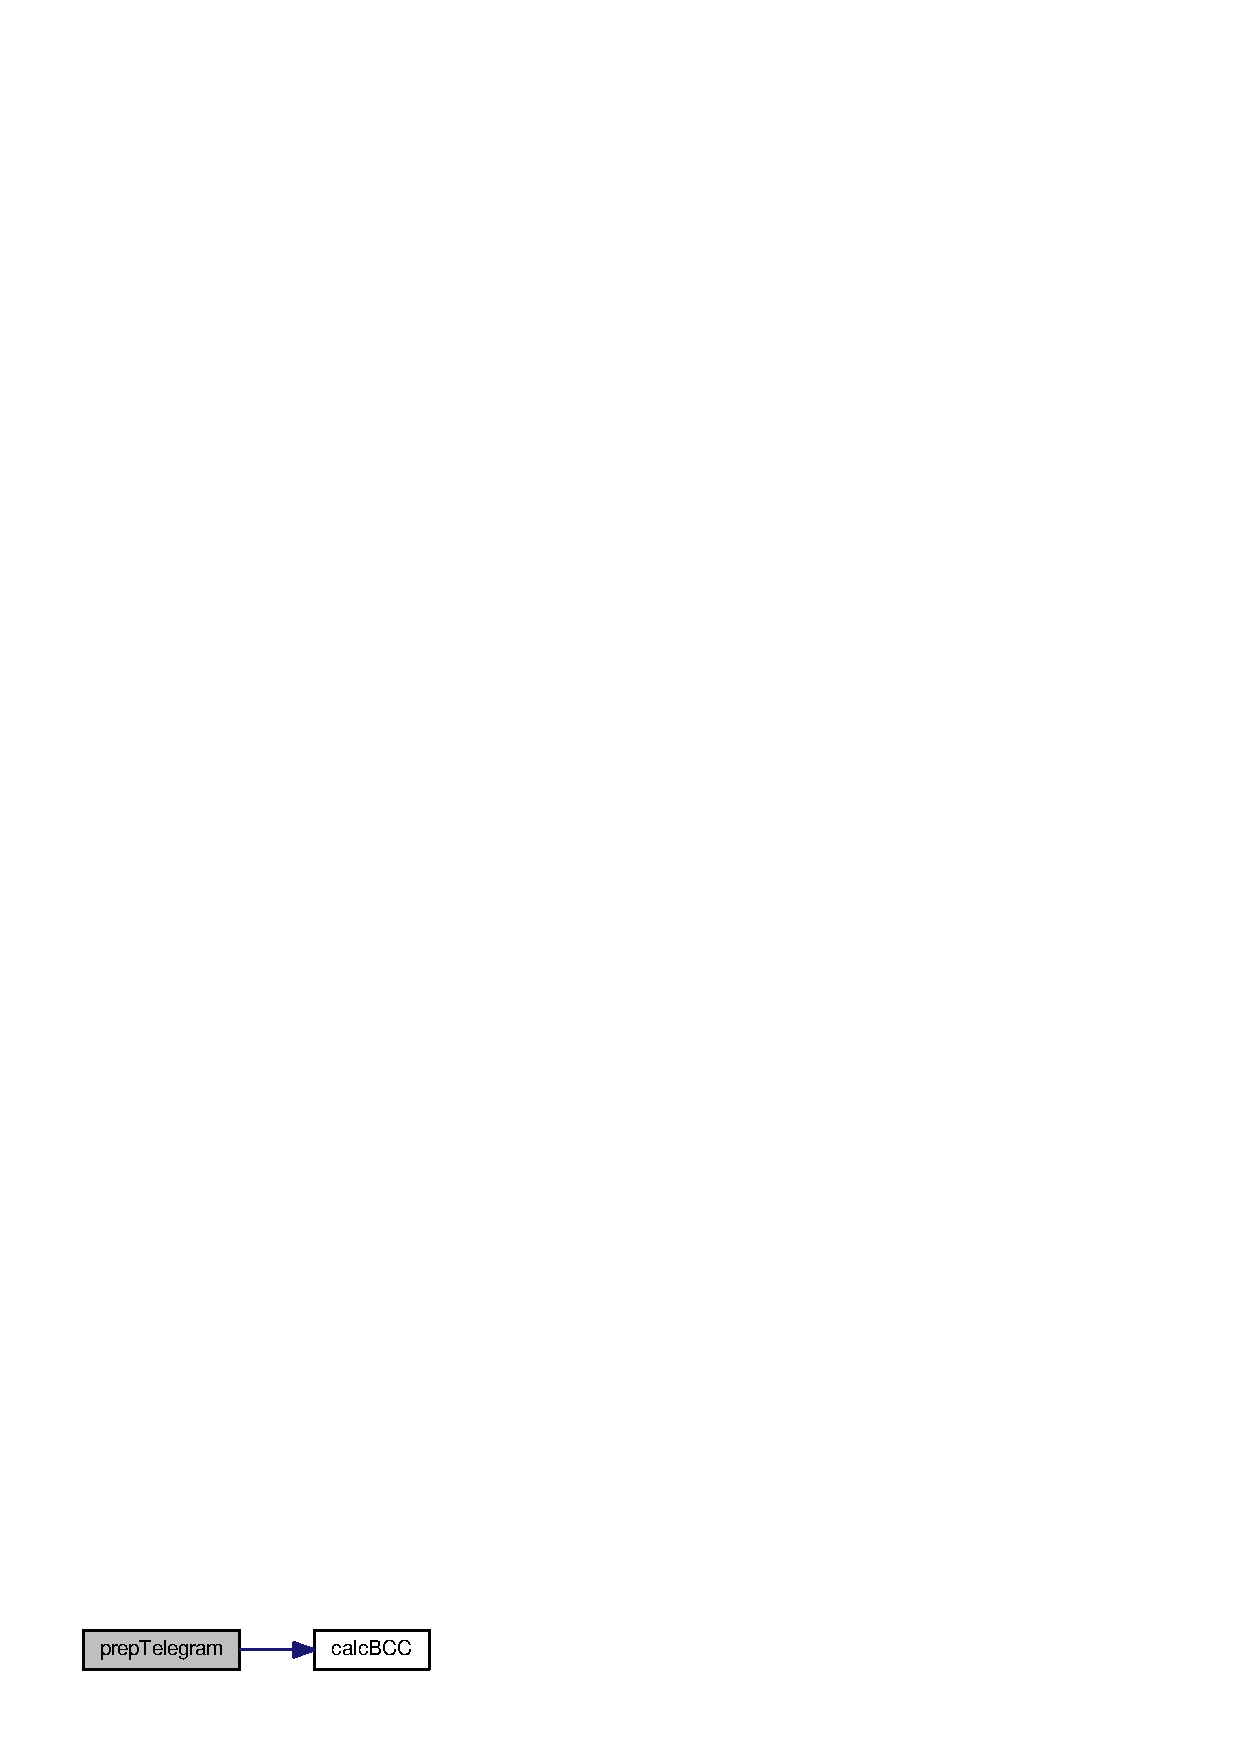
\includegraphics[width=210pt]{usscalc_8c_ac734b72553a80042ac173bfebf6b5185_cgraph}
\end{center}
\end{figure}



\section{U\+:/\+I\+C\+T/7th\+\_\+semester/bpri2/code/my\+Ethernut/rs485/src/usscalc.h File Reference}
\label{usscalc_8h}\index{U\+:/\+I\+C\+T/7th\+\_\+semester/bpri2/code/my\+Ethernut/rs485/src/usscalc.\+h@{U\+:/\+I\+C\+T/7th\+\_\+semester/bpri2/code/my\+Ethernut/rs485/src/usscalc.\+h}}
{\ttfamily \#include \char`\"{}my\+Uart.\+h\char`\"{}}\\*
Include dependency graph for usscalc.\+h\+:\nopagebreak
\begin{figure}[H]
\begin{center}
\leavevmode
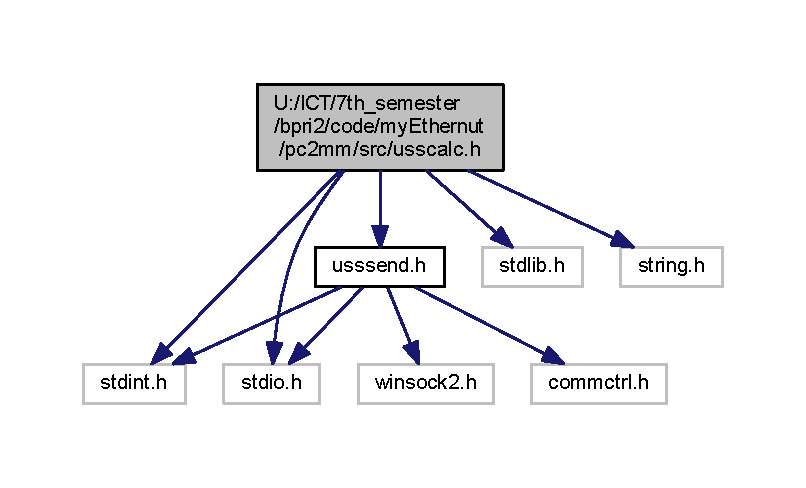
\includegraphics[width=162pt]{usscalc_8h__incl}
\end{center}
\end{figure}
This graph shows which files directly or indirectly include this file\+:\nopagebreak
\begin{figure}[H]
\begin{center}
\leavevmode
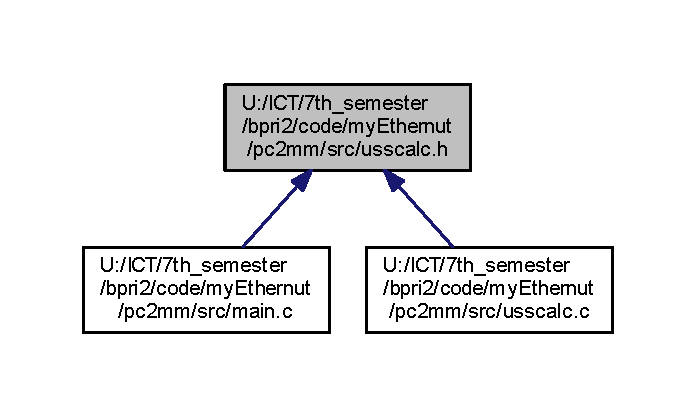
\includegraphics[width=298pt]{usscalc_8h__dep__incl}
\end{center}
\end{figure}
\subsection*{Functions}
\begin{DoxyCompactItemize}
\item 
uint16\+\_\+t {\bf get\+Value} (uint16\+\_\+t my\+Param)
\item 
void {\bf get\+All\+Values} (uint16\+\_\+t $\ast$my\+Param\+Arr, uint8\+\_\+t length)
\end{DoxyCompactItemize}
\subsection*{Variables}
\begin{DoxyCompactItemize}
\item 
uint8\+\_\+t {\bf my\+Telegram} [14]
\end{DoxyCompactItemize}


\subsection{Function Documentation}
\index{usscalc.\+h@{usscalc.\+h}!get\+All\+Values@{get\+All\+Values}}
\index{get\+All\+Values@{get\+All\+Values}!usscalc.\+h@{usscalc.\+h}}
\subsubsection[{get\+All\+Values(uint16\+\_\+t $\ast$my\+Param\+Arr, uint8\+\_\+t length)}]{\setlength{\rightskip}{0pt plus 5cm}void get\+All\+Values (
\begin{DoxyParamCaption}
\item[{uint16\+\_\+t $\ast$}]{my\+Param\+Arr, }
\item[{uint8\+\_\+t}]{length}
\end{DoxyParamCaption}
)}\label{usscalc_8h_ad7a9eba4da373dcceca0624ff97121d4}


Definition at line 106 of file usscalc.\+c.



References get\+Value().



Referenced by main().



Here is the call graph for this function\+:\nopagebreak
\begin{figure}[H]
\begin{center}
\leavevmode
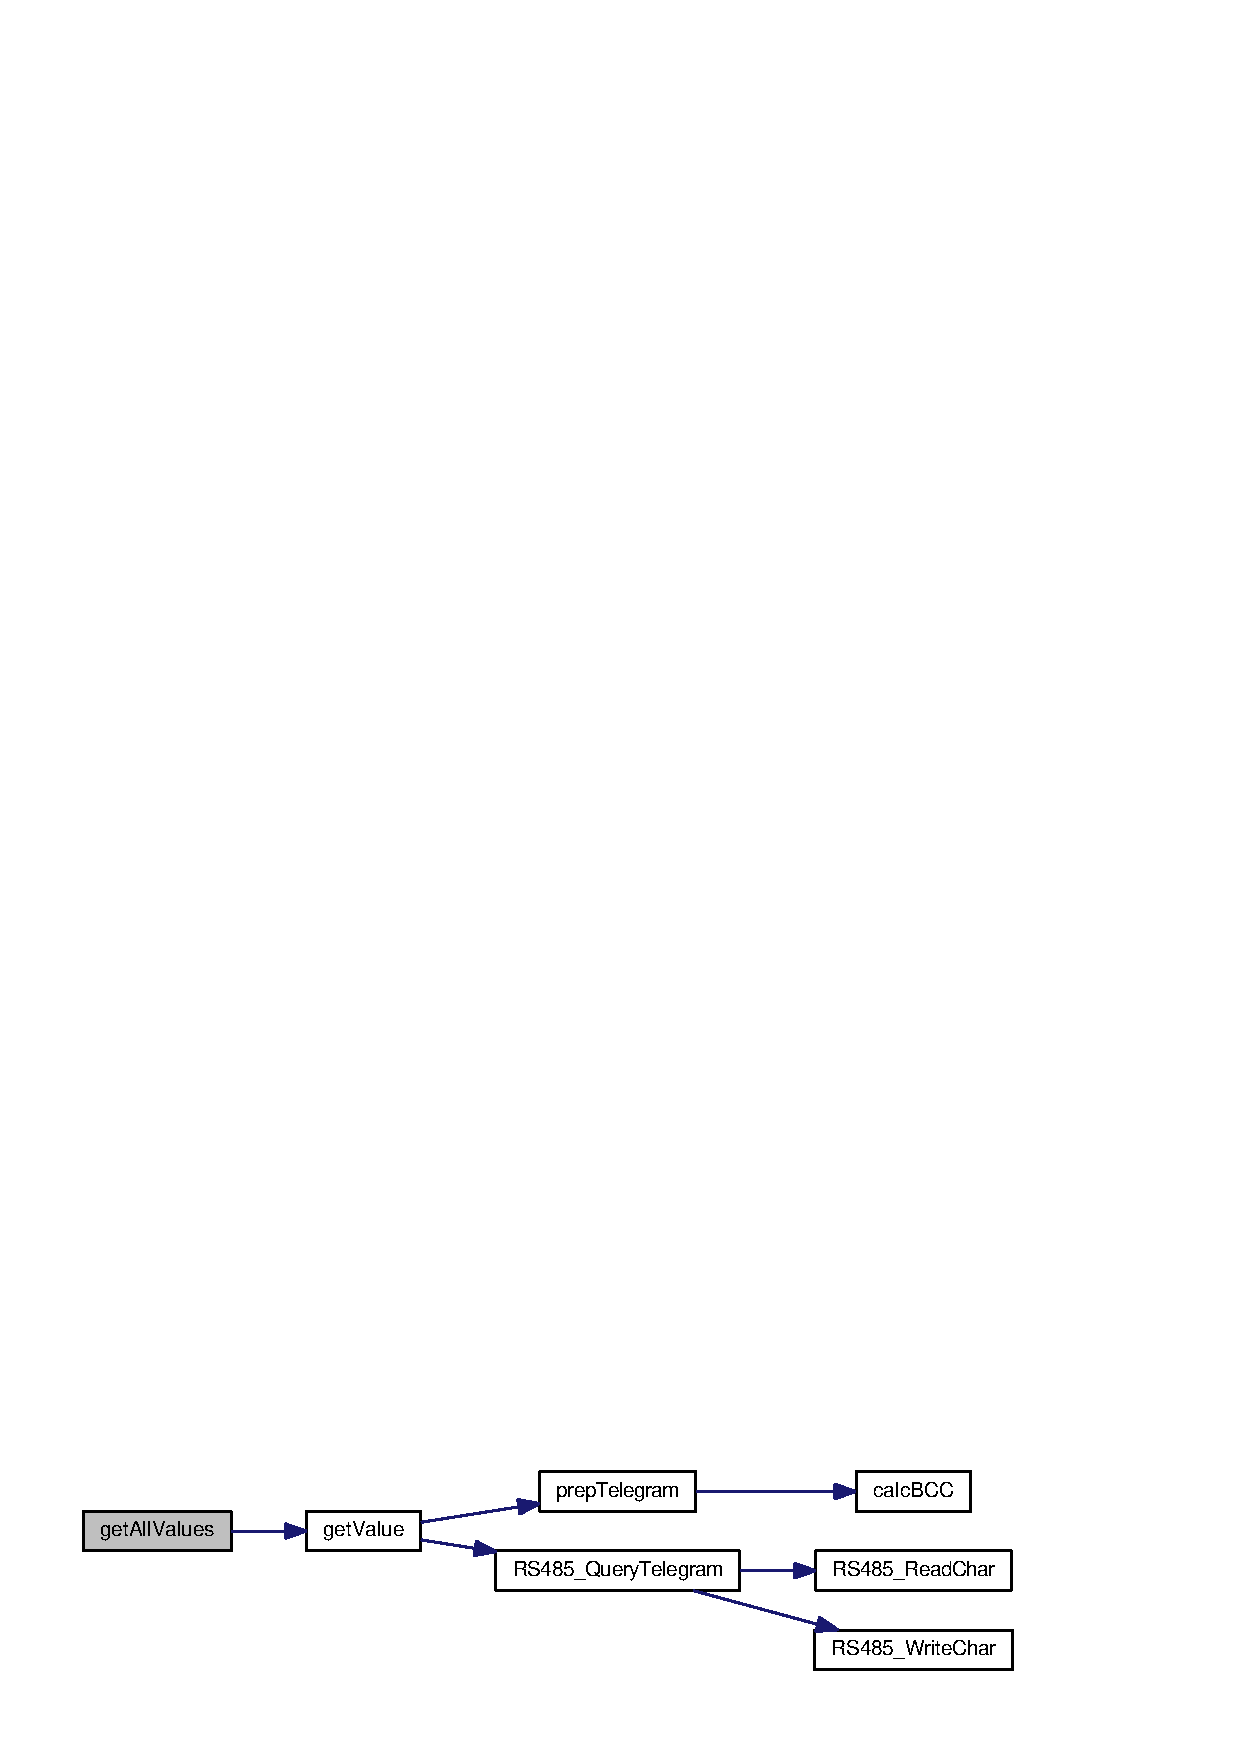
\includegraphics[width=350pt]{usscalc_8h_ad7a9eba4da373dcceca0624ff97121d4_cgraph}
\end{center}
\end{figure}


\index{usscalc.\+h@{usscalc.\+h}!get\+Value@{get\+Value}}
\index{get\+Value@{get\+Value}!usscalc.\+h@{usscalc.\+h}}
\subsubsection[{get\+Value(uint16\+\_\+t my\+Param)}]{\setlength{\rightskip}{0pt plus 5cm}uint16\+\_\+t get\+Value (
\begin{DoxyParamCaption}
\item[{uint16\+\_\+t}]{my\+Param}
\end{DoxyParamCaption}
)}\label{usscalc_8h_a0d092db893cddedce1266d2971f2cd7f}


Definition at line 100 of file usscalc.\+c.



References my\+Telegram, prep\+Telegram(), and R\+S485\+\_\+\+Query\+Telegram().



Referenced by get\+All\+Values().



Here is the call graph for this function\+:\nopagebreak
\begin{figure}[H]
\begin{center}
\leavevmode
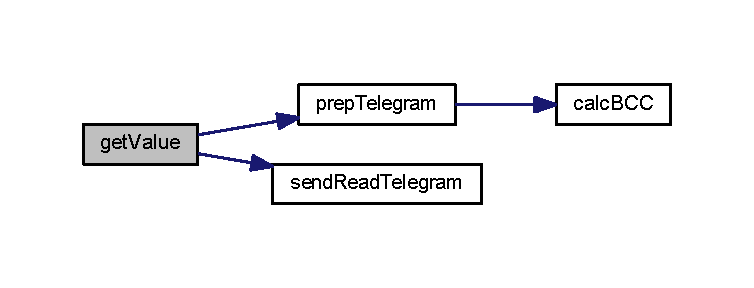
\includegraphics[width=350pt]{usscalc_8h_a0d092db893cddedce1266d2971f2cd7f_cgraph}
\end{center}
\end{figure}




\subsection{Variable Documentation}
\index{usscalc.\+h@{usscalc.\+h}!my\+Telegram@{my\+Telegram}}
\index{my\+Telegram@{my\+Telegram}!usscalc.\+h@{usscalc.\+h}}
\subsubsection[{my\+Telegram}]{\setlength{\rightskip}{0pt plus 5cm}uint8\+\_\+t my\+Telegram[14]}\label{usscalc_8h_ace4b9a76218fd1cc485563419811a46b}


Definition at line 6 of file usscalc.\+h.



Referenced by calc\+B\+C\+C(), get\+Value(), prep\+Telegram(), and R\+S485\+\_\+\+Query\+Telegram().


\hypertarget{usssend_8c}{}\section{U\+:/\+I\+C\+T/7th\+\_\+semester/bpri2/code/my\+Ethernut/pc2mm/src/usssend.c File Reference}
\label{usssend_8c}\index{U\+:/\+I\+C\+T/7th\+\_\+semester/bpri2/code/my\+Ethernut/pc2mm/src/usssend.\+c@{U\+:/\+I\+C\+T/7th\+\_\+semester/bpri2/code/my\+Ethernut/pc2mm/src/usssend.\+c}}
{\ttfamily \#include \char`\"{}usssend.\+h\char`\"{}}\\*
Include dependency graph for usssend.\+c\+:
\nopagebreak
\begin{figure}[H]
\begin{center}
\leavevmode
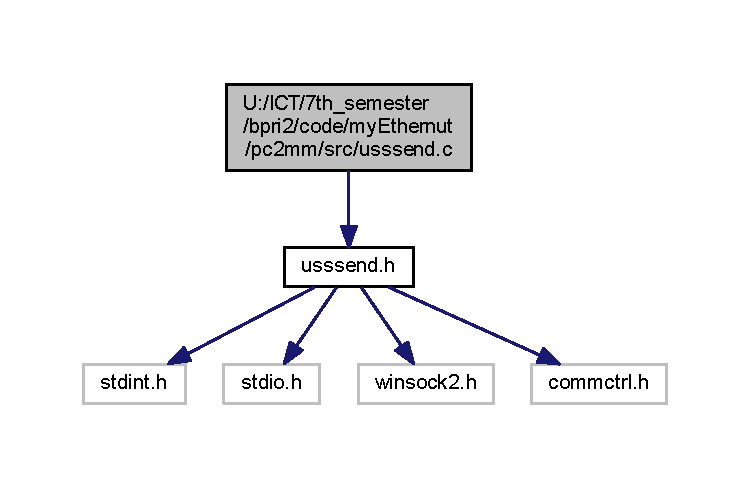
\includegraphics[width=350pt]{usssend_8c__incl}
\end{center}
\end{figure}
\subsection*{Functions}
\begin{DoxyCompactItemize}
\item 
\hyperlink{usscalc_8h_aba7bc1797add20fe3efdf37ced1182c5}{uint8\+\_\+t} $\ast$ \hyperlink{usssend_8c_ac6889b05046a046c3375fa814ea6d609}{send\+Read\+Telegram} (\hyperlink{usscalc_8h_aba7bc1797add20fe3efdf37ced1182c5}{uint8\+\_\+t} $\ast$\hyperlink{usscalc_8h_ace4b9a76218fd1cc485563419811a46b}{my\+Telegram})
\end{DoxyCompactItemize}


\subsection{Function Documentation}
\hypertarget{usssend_8c_ac6889b05046a046c3375fa814ea6d609}{}\index{usssend.\+c@{usssend.\+c}!send\+Read\+Telegram@{send\+Read\+Telegram}}
\index{send\+Read\+Telegram@{send\+Read\+Telegram}!usssend.\+c@{usssend.\+c}}
\subsubsection[{send\+Read\+Telegram(uint8\+\_\+t $\ast$my\+Telegram)}]{\setlength{\rightskip}{0pt plus 5cm}{\bf uint8\+\_\+t}$\ast$ send\+Read\+Telegram (
\begin{DoxyParamCaption}
\item[{{\bf uint8\+\_\+t} $\ast$}]{my\+Telegram}
\end{DoxyParamCaption}
)}\label{usssend_8c_ac6889b05046a046c3375fa814ea6d609}

\hypertarget{usssend_8h}{}\section{U\+:/\+I\+C\+T/7th\+\_\+semester/bpri2/code/my\+Ethernut/pc2mm/src/usssend.h File Reference}
\label{usssend_8h}\index{U\+:/\+I\+C\+T/7th\+\_\+semester/bpri2/code/my\+Ethernut/pc2mm/src/usssend.\+h@{U\+:/\+I\+C\+T/7th\+\_\+semester/bpri2/code/my\+Ethernut/pc2mm/src/usssend.\+h}}
{\ttfamily \#include $<$stdint.\+h$>$}\\*
{\ttfamily \#include $<$stdio.\+h$>$}\\*
{\ttfamily \#include $<$winsock2.\+h$>$}\\*
{\ttfamily \#include $<$commctrl.\+h$>$}\\*
Include dependency graph for usssend.\+h\+:
\nopagebreak
\begin{figure}[H]
\begin{center}
\leavevmode
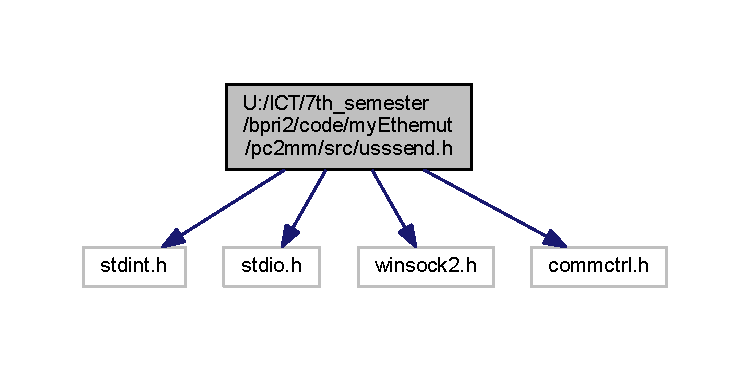
\includegraphics[width=350pt]{usssend_8h__incl}
\end{center}
\end{figure}
This graph shows which files directly or indirectly include this file\+:
\nopagebreak
\begin{figure}[H]
\begin{center}
\leavevmode
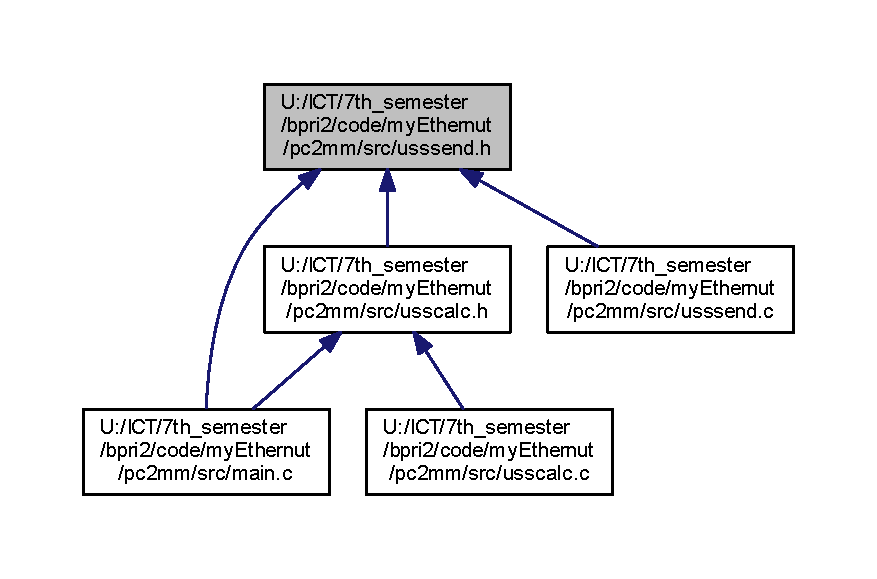
\includegraphics[width=350pt]{usssend_8h__dep__incl}
\end{center}
\end{figure}
\subsection*{Functions}
\begin{DoxyCompactItemize}
\item 
\hyperlink{usscalc_8h_aba7bc1797add20fe3efdf37ced1182c5}{uint8\+\_\+t} $\ast$ \hyperlink{usssend_8h_ac6889b05046a046c3375fa814ea6d609}{send\+Read\+Telegram} (\hyperlink{usscalc_8h_aba7bc1797add20fe3efdf37ced1182c5}{uint8\+\_\+t} $\ast$\hyperlink{usscalc_8h_ace4b9a76218fd1cc485563419811a46b}{my\+Telegram})
\end{DoxyCompactItemize}


\subsection{Function Documentation}
\hypertarget{usssend_8h_ac6889b05046a046c3375fa814ea6d609}{}\index{usssend.\+h@{usssend.\+h}!send\+Read\+Telegram@{send\+Read\+Telegram}}
\index{send\+Read\+Telegram@{send\+Read\+Telegram}!usssend.\+h@{usssend.\+h}}
\subsubsection[{send\+Read\+Telegram(uint8\+\_\+t $\ast$my\+Telegram)}]{\setlength{\rightskip}{0pt plus 5cm}{\bf uint8\+\_\+t}$\ast$ send\+Read\+Telegram (
\begin{DoxyParamCaption}
\item[{{\bf uint8\+\_\+t} $\ast$}]{my\+Telegram}
\end{DoxyParamCaption}
)}\label{usssend_8h_ac6889b05046a046c3375fa814ea6d609}

%--- End generated contents ---

% Index
\backmatter
\newpage
\phantomsection
\clearemptydoublepage
\addcontentsline{toc}{chapter}{Index}
\printindex

\end{document}
